\section{Raspberry Pi 3}
\label{sec:raspi3}
The Raspberry Pi is a high-performance single-board computer designed to educate
and solve real-world problems. This small computer supports a camera module that
uses a Sony IMX219 8 mega-pixel CMOS sensor.
%
\subsection{Specification}
\label{ssec:raspispecification}
The Raspberry Pi Foundation provides low-cost, high-performance single-board 
Raspberry Pi computers to educate and solve real-world problems.  As of early
2016, over 8 million Raspberry Pi's had been sold, making it one of the most
popular single-board computers on the market.\cite{upton2016raspberry}\\ The
Raspberry Pi credit-card-sized computer supports several accessories, including
a camera module containing the Sony IMX219 sensor. This computer and camera
configuration is of particular interest since it can provide raw-data format
imagery that can be used for a multitude of applications, including computer
vision, biophotonics, medical testing, remote sensing, astronomy, improved image
quality, high dynamic range (HDR) imaging, and security monitoring. The
Raspberry Pi 3 is the third generation single board Raspberry Pi computer and
became available to consumers in February 2016. \\Some of the more significant
Raspberry Pi attributes, including interfaces, are described in Table
\ref{tab:rapberryattributes}. At the time of this writing, a Raspberry Pi 3 sold
for about \$35 USD and the V2.1 camera module sold for approximately \$25
USD.\cite{upton2016raspberry, raspberrycam}\\
The Raspberry Pi Foundation provides several operating systems for the 
Raspberry Pi 3, including Raspbian and a Debian-based Linux distribution, as 
well as third-party Ubuntu, Windows 10 IOT Core, RISC OS, and specialized 
distributions for download.\cite{10.1117/1.JEI.26.1.013014}
%
\begin{table}[htb]
\centering
	\caption{Raspberry Pi 3 computer attributes.}
	\label{tab:rapberryattributes}
	\begin{tabular}{l}
		\hline
		CPU 1.2 \si{\giga\hertz} 64-bit ARM Cortex-A53 \\
		1 GB of RAM LPDDR2 (900 \si{\mega\hertz}) \\
		Wireless N and Blue-tooth 4.1 communication\\
		Four USB ports\\
		HDMI interface\\
		Ethernet port\\
		MicroSD card slot\\
		40 GPIO pins\\
		Camera interface\\
		Composite video audio jack\\
		\hline
\end{tabular}
\end{table}
%
\section{Raspberry Pi, Camera Board V2}
\label{sec:raspicam}
The camera is based on the Sony IMX219 silicon CMOS back-lit sensor and produces
8 mega-pixel images that are $3280 \times 2464$ pixels in size. \\
The IMX219 sensor operates in the visible spectral range from 400 to 700 \si{\nano\meter}).\cite{raspberrycam2}
Sensor specifications are detailed in Table \ref{tab:raspicamspec}.
%
\begin{table}[!h]
	\centering
	\caption{Sony IMX219 sensor chip specifications.}
	\label{tab:raspicamspec}
	\begin{tabular}{l l}
		\hline
		\textbf{Sensor parameter}			& 	\textbf{Specification}\\
		\hline
		Image sensor type		&	Back-lit CMOS\\
		Image size				&	Diagonal 4.60 \si{\milli\meter} (type 1/4.0)\\
		Number of active pixels	&	3280 (H) $\times$ 2464 (V) $\sim$ 8.08 mega-pixels\\
		Chip size				&	5.095 \si{\milli\meter} (H) $\times$ 4.930 \si{\milli\meter}(V) (w/ Scribe)\\	
		Unit cell size (pixel) 	&	1.12 \si{\micro\meter} (H) $\times$ 1.12 \si{\micro\meter}(V)\\
		Substrate material		&	Silicon\\
		Bit depth				&	10-bit A/D converter on chip\\
		Data output				&	CSI2 serial data output (selection of 4 lane/ 2 lane)\\
		Communication			&	2-wire serial communication circuit on chip\\
		Max full-frame frame rate &	30 frames/s \\
		Pixel rate 				&	280 mega-pixel/s (all-pixels mode)\\
		Data rate				&	Max. 755 Mbps/lane (at 4 lane), 912 Mbps / lane(at 2 lane)\\
		\hline
	\end{tabular}
\end{table}
%
\subsection{Specification}
\label{ssec:raspcamspecification}
The V2 camera module operates at a fixed focal length (3.04 \si{\milli\meter})
and single $f$-number (F$2.0$) typically focused from the near-field to
infinity. Images can be captured at ISO settings between 100 and 800 in manually
set increments of 100 (although not verified above 600 in this investigation)
and camera exposure times between \SI{9}{\micro\second} and 6 \si{\second} using
a rolling shutter. Some of the more significant camera specifications are shown
in Table \ref{tab:raspicamspec2}. In addition to still photos, the Raspberry Pi
Sony IMX219 sensor supports a cropped 1080p format at 30 frames per second (fps)
and full-frame imaging video at up to 15 fps, but not in raw-data format. The
entire camera board is small 25 \si{\milli\meter} $\times$ 25 \si{\milli\meter}
$\times$ 9 \si{\milli\meter} and weighing about $3$ \si{\gram}. It connects
directly to the Raspberry Pi 3 through a 15 pin mobile industry processor
interface (MIPI) camera serial interface and is shown alongside a Raspberry Pi 3
in Figure \ref{fig:boardcam}.\cite{upton2016raspberry, raspberrycam}
%
\begin{table}[htb]
	\centering
	\caption{Raspberry Pi camera.}
	\label{tab:raspicamspec2}
	\begin{tabular}{l l}
		\hline
		\textbf{Camera parameter}			& 	\textbf{Specification}\\
		\hline
		Lens focal length 	& 	3.04 \si{\milli\meter}	\\
		$f$-number			&	2.0	\\
		Instantaneous field of view	&	0.368 \si{\milli\radian}\\
		Full-frame field of view & 59.17 \si{\degree}(H) $\times$ 58.3 \si{\degree} (V)\\
		\hline
	\end{tabular}
\end{table}
%

\begin{figure}[htb]
	\centering
    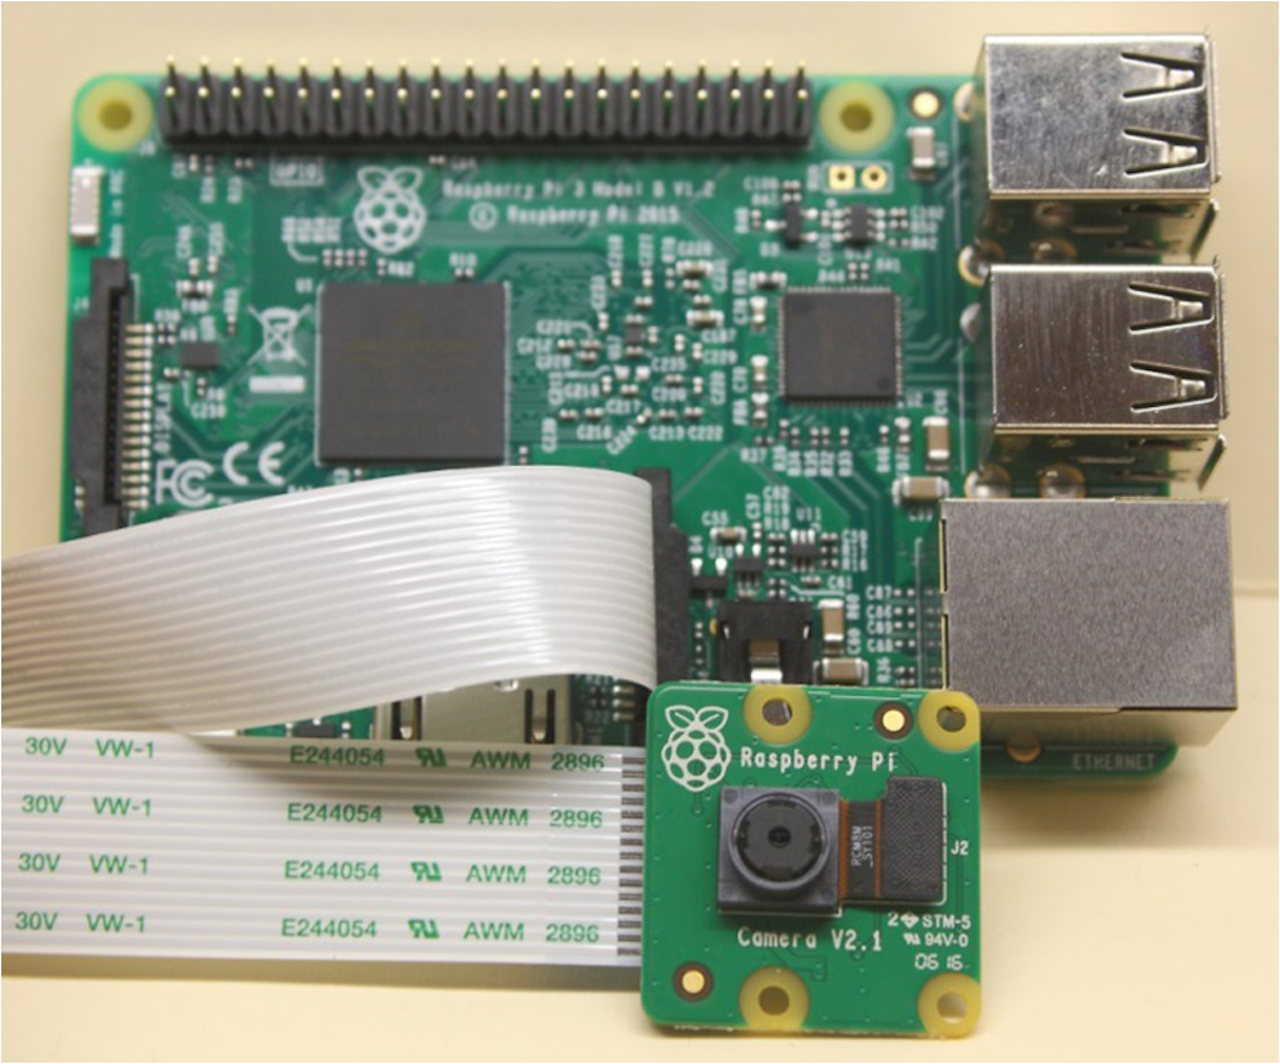
\includegraphics[width=0.80\textwidth]{JEI_26_1_013014_f001.png}
    \caption{Raspberry Pi 3 and camera module V2.1.}
    \label{fig:boardcam}
\end{figure}